% UTF-8 encoding
% Compile with latex+dvipdfmx, pdflatex, xelatex or lualatex

\documentclass[UTF8]{ctexart}
\usepackage{graphicx}
\usepackage{amssymb}
\usepackage{amsmath}
\usepackage{subfigure}
\usepackage{geometry}
\usepackage{caption}

\newcommand{\true}{{\rm T}}
\newcommand{\false}{{\rm F}}
\newcommand{\snatural}{\mathbb{N}}
\newcommand{\sinteger}{\mathbb{Z}}
\newcommand{\srational}{\mathbb{Q}}
\newcommand{\sreal}{\mathbb{R}}
\newcommand{\card}{\rm{card}}
\newcommand{\modt}{\text{mod }}
\newcommand{\ran}{{\rm ran}}
\newcommand{\dom}{{\rm dom}}

\title{离散数学——第十二周作业}
\author{计83  刘轩奇  2018011025}
\date{2019.11.29}

\geometry{left=2.0cm, right=2.0cm, top=2.5cm, bottom=2.5cm}

\begin{document}

\maketitle

\paragraph{10.13} \label{10.13}
    对$A$到$B$的关系$R$,$a \in A$,定义$B$的一个子集$R(a)=\{b|aRb\}$,在$C=\{-4,-3,-2,-1,0,1,2,3,4\}$上定义$R= \{ \langle x,y \rangle |x \langle y \} $, $S= \{ \langle x,y \rangle |x-1 < y < x+2 \} $, $ \true = \{ \langle x,y \rangle |x^2 \le y \} $,写出集合$R(0), R(1), S(0), S(-1), \true (0), \true (-1).$

\paragraph{解}
    \begin{align*}
        R(0) & = \{ 1,2,3,4 \} \\
        R(1) & = \{ 2,3,4 \} \\
        S(0) & = \{ 0,1 \} \\
        S(-1) & = \{ -1, 0 \} \\
        T(0) & = \{ 0,1,2,3,4 \} \\
        T(1) & = \{ 1,2,3,4 \} 
    \end{align*}

\paragraph{10.14} \label{10.14}
    对命题:“集合$A$上的一个关系$R$,如果是对称的和传递的,就一定是自反的。因为$xRy$和$yRx$蕴含$xRx$。”依据定义找出错误。在$\{1,2,3\}$上构造一个关系,它是对称的和传递的,但不是自反的。

\paragraph{答}
    $R$中可能不存在任何一个$y$使得$xRy,yRx$成立,因而$xRx$不一定成立。

    例如空关系是对称且传递的,但不是自反的。

\paragraph{10.15} \label{10.15}
    对集合$A=\{1,2,3\}$上,下列8种关系图(图见书第189面,此处省略),说明每个关系具有的性质。

\paragraph{解} 如表 10-15 所示。
    \begin{table}[htb]
        \centering
        \begin{tabular}{ccccc}
        关系    & 自反性          & 反自反性         & 对称性          & 传递性          \\
        $R_1$ & $\times$     & $\times$     & $\times$     & $\times$     \\
        $R_2$ & $\times$     & $\times$     & $\checkmark$ & $\checkmark$ \\
        $R_3$ & $\checkmark$ & $\times$     & $\checkmark$ & $\checkmark$ \\
        $R_4$ & $\checkmark$ & $\times$     & $\times$     & $\checkmark$ \\
        $R_5$ & $\times$     & $\times$     & $\times$     & $\times$     \\
        $R_6$ & $\times$     & $\checkmark$ & $\checkmark$ & $\times$     \\
        $R_7$ & $\times$     & $\checkmark$ & $\checkmark$ & $\times$     \\
        $R_8$ & $\checkmark$ & $\times$     & $\checkmark$ & $\times$    
        \end{tabular}
        \caption*{表 10-15}
    \end{table}

\paragraph{10.16} \label{10.16}
    对集合$A=\{1,2,3,\cdots,10\}$,$A$上的关系$R$和$S$各有什么性质。
    $$R= \{ \langle x,y \rangle |x+y=10 \}$$
    $$S= \{ \langle x,y \rangle |x+y\text { 是偶数 } \} $$

\paragraph{答}$R:$对称性;$S:$自反性、对称性、传递性。

\paragraph{10.17} \label{10.17}
    对$A$上的关系$R$,证明:
    
    (1) $R\text{是自反的} \Longleftrightarrow I_A\subseteq R$

\paragraph{证} (1)
    \subparagraph{充分性} 若$R$是自反的,则$ ( \forall x)(x \in A \rightarrow (x,x) \in R)$
        $$ \langle x,y \rangle \in I_A \Longleftrightarrow x \in A \land x = y \Longrightarrow \langle x,y \rangle \in R \land x=y$$
        $$\therefore I_A \subseteq R$$
    \subparagraph{必要性} 若$I_A \subseteq R$
        $$x \in A \Longrightarrow \langle x,x \rangle \in I_A \Longrightarrow \langle x,x \rangle \in R$$
        
        则$R$是自反的。

\paragraph{10.18} \label{10.18}
    对$A$上的关系$R_1$和$R_2$,判定下列命题的真假。真的证明之,假的举反例。

    (1) 若$R_1$和$R_2$是自反的,则$R_1 \circ R_2$是自反的。

    (3) 若$R_1$和$R_2$是对称的,则$R_1 \circ R_2$是对称的。

\paragraph{解}

    (1) 真。
    $$x \in A \Longrightarrow \langle x,x \rangle \in R_1 \land \langle x,x \rangle \in R_2 \Longrightarrow \langle x,x \rangle \in R_1 \circ R_2$$

    (3) 假。反例:$$A= \{ 1,2,3 \} , R_1= \{ \langle 2,3 \rangle , \langle 3,2 \rangle \} , R_2 = \{ \langle 1,2 \rangle , \langle 2,1 \rangle \} , R_1 \circ R_2 = \{ \langle 1,3 \rangle \} $$不是对称的。

\paragraph{10.19} \label{10.19}
    对集合$A=\{1,2,3\}$,给出$A$上的关系$R$的例子,使它具有下列性质。
    
    (1) 对称的且反对称的且传递的。

    (3) 不是对称的且不是反对称的且传递的。

\paragraph{答}

    (1) $R = I_A = \{ \langle 1,1 \rangle , \langle 2,2 \rangle , \langle 3,3 \rangle \} $

    (3) $R = \{ \langle 1,1 \rangle , \langle 1,2 \rangle , \langle 2,1 \rangle , \langle 2,2 \rangle , \langle 1,3 \rangle , \langle 2,3 \rangle \} $

\paragraph{10.20} \label{10.20}
    对集合$A= \{ 1,2,3,4 \} $,$A$上的关系$R$为
    $$R= \{ \langle 1,2 \rangle , \langle 4,3 \rangle , \langle 2,2 \rangle , \langle 2,1 \rangle , \langle 3,1 \rangle \} $$
    说明$R$不是传递的。构造$A$上的关系$R_1$,使$R\subseteq R_1$且$R_1$是传递的。

\paragraph{解}
    $ \langle 1,2 \rangle \in R, \langle 2,1 \rangle \in R, $但$ \langle 1,1 \rangle \notin R$则$R$不是传递的。
    $$R_1 = \{ \langle 1,1 \rangle , \langle 1,2 \rangle , \langle 2,1 \rangle , \langle 2,2 \rangle , \langle 3,1 \rangle , \langle 3,2 \rangle , \langle 4,1 \rangle , \langle 4,2 \rangle , \langle 4,3 \rangle \} $$

\paragraph{10.22} \label{10.22}
    对集合$A= \{ a,b,c,d \} $上的两个关系
    \begin{align*}
        R_1 & = \{ \langle a,a \rangle , \langle a,b \rangle , \langle b,d \rangle \} \\
        R_2 & = \{ \langle a,d \rangle , \langle b,c \rangle , \langle b,d \rangle , \langle c,b \rangle \} 
    \end{align*}
    求$R_1 \circ R_2$,$R_2 \circ R_1$,$R_1^2$,$R_2^2$。

\paragraph{解}
    \begin{align*}
        R_1 \circ R_2 & = \{ \langle c,d \rangle \} \\
        R_2 \circ R_1 & = \{ \langle a,d \rangle , \langle a,c \rangle \} \\
        R_1^2 & = \{ \langle a,a \rangle , \langle a,b \rangle , \langle a,d \rangle \} \\
        R_2^2 & = \{ \langle b,b \rangle , \langle c,c \rangle , \langle c,d \rangle \} 
    \end{align*}

\paragraph{10.24} \label{10.24}
    $A=\{a,b,c,d,e\}$上的关系$R$的关系图如下。给出$r(R),s(R),t(R)$的关系图。

\paragraph{解}
    如图10-24所示。
    \begin{figure}[!htb]
        \centering
        \begin{minipage}[t]{0.584\textwidth}
        \centering
        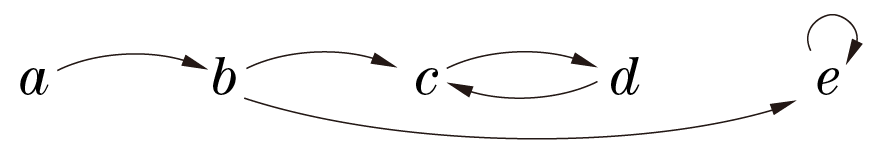
\includegraphics[width=1\textwidth]{10-24-o.png}
        \caption*{(a) $R$}
        \end{minipage}
        \\
        \begin{minipage}[t]{0.591\textwidth}
        \centering
        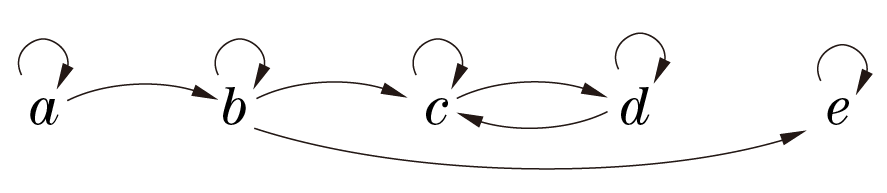
\includegraphics[width=1\textwidth]{10-24-r.png}
        \caption*{(b) $r(R)$}
        \end{minipage}
        \\
        \begin{minipage}[t]{0.581\textwidth}
        \centering
        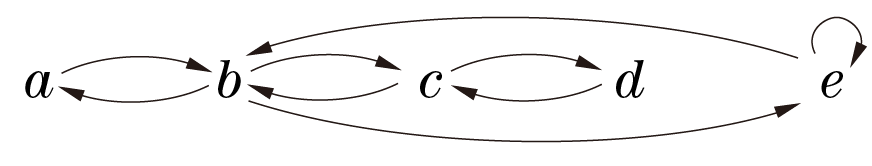
\includegraphics[width=1\textwidth]{10-24-s.png}
        \caption*{(c) $s(R)$}
        \end{minipage}
        \\
        \begin{minipage}[t]{0.583\textwidth}
        \centering
        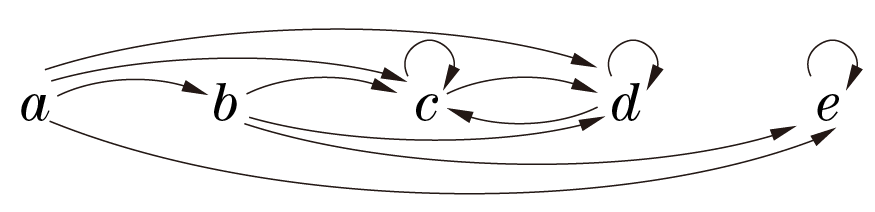
\includegraphics[width=1\textwidth]{10-24-t.png}
        \caption*{(d) $t(R)$}
        \end{minipage}
        \caption*{图 10-24}
    \end{figure}
        
\paragraph{10.27} \label{10.27}
    对$A=\{a,b,c,d\}$上的关系
    $$R = \{ \langle a,b \rangle , \langle b,a \rangle , \langle b,c \rangle , \langle c,d \rangle \} $$
    
    (1) 分别用矩阵运算和作图法求$r(R),s(R),t(R)$。

    (2) 用Warshall算法求$t(R)$。

\paragraph{解}

    (1) 矩阵运算法:
    \begin{align*}
        M(R) & = \begin{bmatrix}
            0 & 1 & 0 & 0 \\
            1 & 0 & 1 & 0 \\
            0 & 0 & 0 & 1 \\
            0 & 0 & 0 & 0
        \end{bmatrix} \\
        M(r(R)) = M(R \cup I_A) & = \begin{bmatrix}
            1 & 1 & 0 & 0 \\
            1 & 1 & 1 & 0 \\
            0 & 0 & 1 & 1 \\
            0 & 0 & 0 & 1
        \end{bmatrix} \\
        M(s(R)) = M(R \cup R^{-1}) & = \begin{bmatrix}
            0 & 1 & 0 & 0 \\
            1 & 0 & 1 & 0 \\
            0 & 1 & 0 & 1 \\
            0 & 0 & 1 & 0
        \end{bmatrix} \\
        M(t(R)) = M(R \cup R^2 \cup R^3 \cup R^4) & = \begin{bmatrix}
            1 & 1 & 1 & 1 \\
            1 & 1 & 1 & 1 \\
            0 & 0 & 0 & 1 \\
            0 & 0 & 0 & 0
        \end{bmatrix}
    \end{align*}
    
    作图法,如图 10-27 所示:
    \begin{figure}[!htb]
        \centering
        \begin{minipage}[t]{0.453\textwidth}
        \centering
        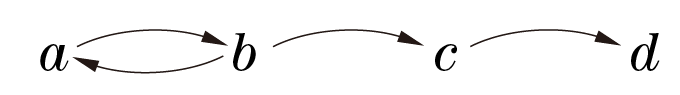
\includegraphics[width=1\textwidth]{10-27-o.png}
        \caption*{(a) $R$}
        \end{minipage}
        \\
        \begin{minipage}[t]{0.454\textwidth}
        \centering
        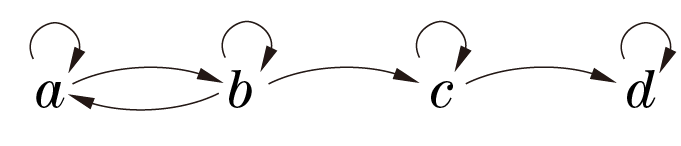
\includegraphics[width=1\textwidth]{10-27-r.png}
        \caption*{(b) $r(R)$}
        \end{minipage}
        \\
        \begin{minipage}[t]{0.443\textwidth}
        \centering
        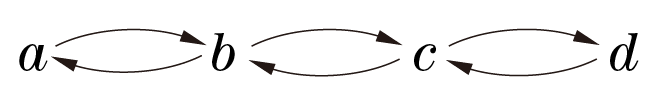
\includegraphics[width=1\textwidth]{10-27-s.png}
        \caption*{(c) $s(R)$}
        \end{minipage}
        \\
        \begin{minipage}[t]{0.458\textwidth}
        \centering
        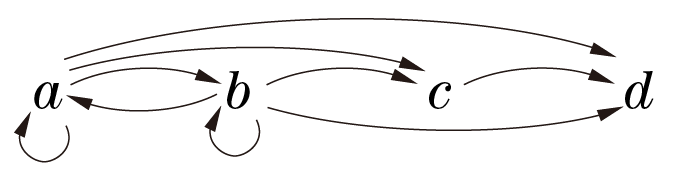
\includegraphics[width=1\textwidth]{10-27-t.png}
        \caption*{(d) $t(R)$}
        \end{minipage}
        \caption*{图 10-27}
    \end{figure}

    以上两种方法均可得
    \begin{align*}
        r(R) & = \{ \langle a,a \rangle , \langle a,b \rangle , \langle b,a \rangle , \langle b,b \rangle , \langle b,c \rangle , \langle c,c \rangle , \langle c,d \rangle , \langle d,d \rangle \} \\
        s(R) & = \{ \langle a,b \rangle , \langle b,a \rangle , \langle b,c \rangle , \langle c,b \rangle , \langle c,d \rangle , \langle d,c \rangle \} \\
        t(R) & = \{ \langle a,a \rangle , \langle a,b \rangle , \langle a,c \rangle , \langle a,d \rangle , \langle b,a \rangle , \langle b,b \rangle , \langle b,c \rangle , \langle b,d \rangle , \langle c,d \rangle \} 
    \end{align*}

    (2) 
    \begin{align*}
        B = M(R) & = \begin{bmatrix}
            0 & 1 & 0 & 0 \\
            1 & 0 & 1 & 0 \\
            0 & 0 & 0 & 1 \\
            0 & 0 & 0 & 0
        \end{bmatrix} \\
        B_1 & = \begin{bmatrix}
            0 & 1 & 0 & 0 \\
            1 & 1 & 1 & 0 \\
            0 & 0 & 0 & 1 \\
            0 & 0 & 0 & 0
        \end{bmatrix} \\
        B_2 & = \begin{bmatrix}
            1 & 1 & 1 & 0 \\
            1 & 1 & 1 & 0 \\
            0 & 0 & 0 & 1 \\
            0 & 0 & 0 & 0
        \end{bmatrix} \\
        B_3 & = \begin{bmatrix}
            1 & 1 & 1 & 1 \\
            1 & 1 & 1 & 1 \\
            0 & 0 & 0 & 1 \\
            0 & 0 & 0 & 0
        \end{bmatrix} \\
        B_4 & = \begin{bmatrix}
            1 & 1 & 1 & 1 \\
            1 & 1 & 1 & 1 \\
            0 & 0 & 0 & 1 \\
            0 & 0 & 0 & 0
        \end{bmatrix} = M(R_+)
    \end{align*}
    $$\therefore t(R) = \{ \langle a,a \rangle , \langle a,b \rangle , \langle a,c \rangle , \langle a,d \rangle , \langle b,a \rangle , \langle b,b \rangle , \langle b,c \rangle , \langle b,d \rangle , \langle c,d \rangle \} $$

\end{document} 